\documentclass{article}

\usepackage[
  top=2cm,
  bottom=2.5cm,
  left=2.5cm,
  right=2.5cm
]{geometry}
\usepackage{arev}
\usepackage[T1]{fontenc}
\usepackage[colorlinks=true, linkcolor=blue, urlcolor=blue]{hyperref}
\usepackage[export]{adjustbox}
\usepackage{graphicx}
\usepackage{subfig}
\setcounter{tocdepth}{3}
\usepackage{booktabs}
\usepackage{tabularx}
\usepackage{graphicx}
\usepackage{xcolor}
\usepackage{amssymb}  % Checkmarks and crosses
\usepackage{pifont}   % Symbols
\newcommand{\cmark}{\textcolor{green}{\ding{51}}}  % checkmark
\newcommand{\xmark}{\textcolor{red}{\ding{55}}}    % cross

\newcommand\imgin[3]{
    \begin{figure*}[htbp]
        \centering
        \includegraphics[width=1.0\textwidth]{images/#1}
        \caption{#2}
        \label{fig:#3}
    \end{figure*}
}

\newcommand\imginin[4]{
    \begin{figure*}[htbp]
        \centering
        \includegraphics[width=#4\textwidth]{images/#1}
        \caption{#2}
        \label{fig:#3}
    \end{figure*}
}
\newcommand\imginrot[5]{
    \begin{figure}[htbp]
        \centering
        \includegraphics[angle=#5, width=#4\textwidth]{images/#1}
        \caption{#2}
        \label{fig:#3}
    \end{figure}
}

\newcommand\imgpairin[8]{
    \begin{figure*}[htbp]
        \centering
        \subfloat[#2]{\includegraphics[angle=#7, width=0.40\textwidth, valign=c]{images/#1}}
        \hspace{0.5cm}
        \subfloat[#4]{\includegraphics[angle=#8, width=0.40\textwidth, valign=c]{images/#3}}
        \caption{#5}
        \label{fig:#6}
    \end{figure*}
}

\begin{document}

% Title
\begin{titlepage}
    \centering
    \vspace*{2cm}
    {\Huge\bfseries Portfolio \par}
    \vspace{2cm}
    {\Large Jackson Russell \par}
    \vspace{1cm}

    % Contact details
    \textbf{Email:} \href{mailto:jackrussell772@gmail.com}{jackrussell772@gmail.com} \\
    \textbf{Phone:} 0434 421 611 \\
    \textbf{LinkedIn:} \href{https://www.linkedin.com/in/jackson-russell-7aa157205/}{LinkedIn} \\ 
    \textbf{GitHub:} \href{https://github.com/jackfruittt}{GitHub} \\

    \vfill

\end{titlepage}

% Table of Contents
\tableofcontents
\newpage


% Include sections
\section*{Introduction}
\addcontentsline{toc}{section}{Introduction}
This is my portfolio showcasing many projects I have completed via work experience or course work throughout my degree which I'm still completing. 
This entire protfolio is written in LaTeX because it's far superior to word (except formatting.. that sucks). You can find the codebase for this 
portolio \href{https://github.com/jackfruittt/Work_Portfolio}{here}. I've tried to keep this portfolio as brief as possible so you don't have to end 
up reading too many pages. If what I've done seems of interest you're more than welcome to contact me using the contact details on the title page and 
check out my LinkedIn and GitHub.
\newpage
\section{RIMA1 and RIMA2: Conditianal Assessment Robotic Tools for Sewer Pipes}

\label{sec:industry}

\textbf{Brief: } RIMA1 [~\ref{fig:rima1}] and RIMA2 [~\ref{fig:rima2}] are two robotic tools developed by the UTS Robotics Institute in collaboration with Sydney Water. They are designed to conditionally assess the pipe walls of sewer 
pipes using Pulse Eddy Current (PEC) Sensors. Both robots operate in the ROS1 framework and are equipped with various sensors such as IMU and RGB-D cameras. Both robots communicate with the base station using VDSL via a 
kevlar braided cable. The subsections will go over more specific tasks I did on RIMA1 and RIMA2 meaning it will exclude things such as general maintenance and repair.

\begin{figure*}[htbp]
    \centering
    \begin{minipage}[t]{0.48\textwidth}
        \centering
        \includegraphics[width=\textwidth]{images/rima1/RIMA1_Physical_Weight_Detatched.jpg}
        \caption{RIMA1}
        \label{fig:rima1}
    \end{minipage}
    \hfill
    \begin{minipage}[t]{0.48\textwidth}
        \centering
        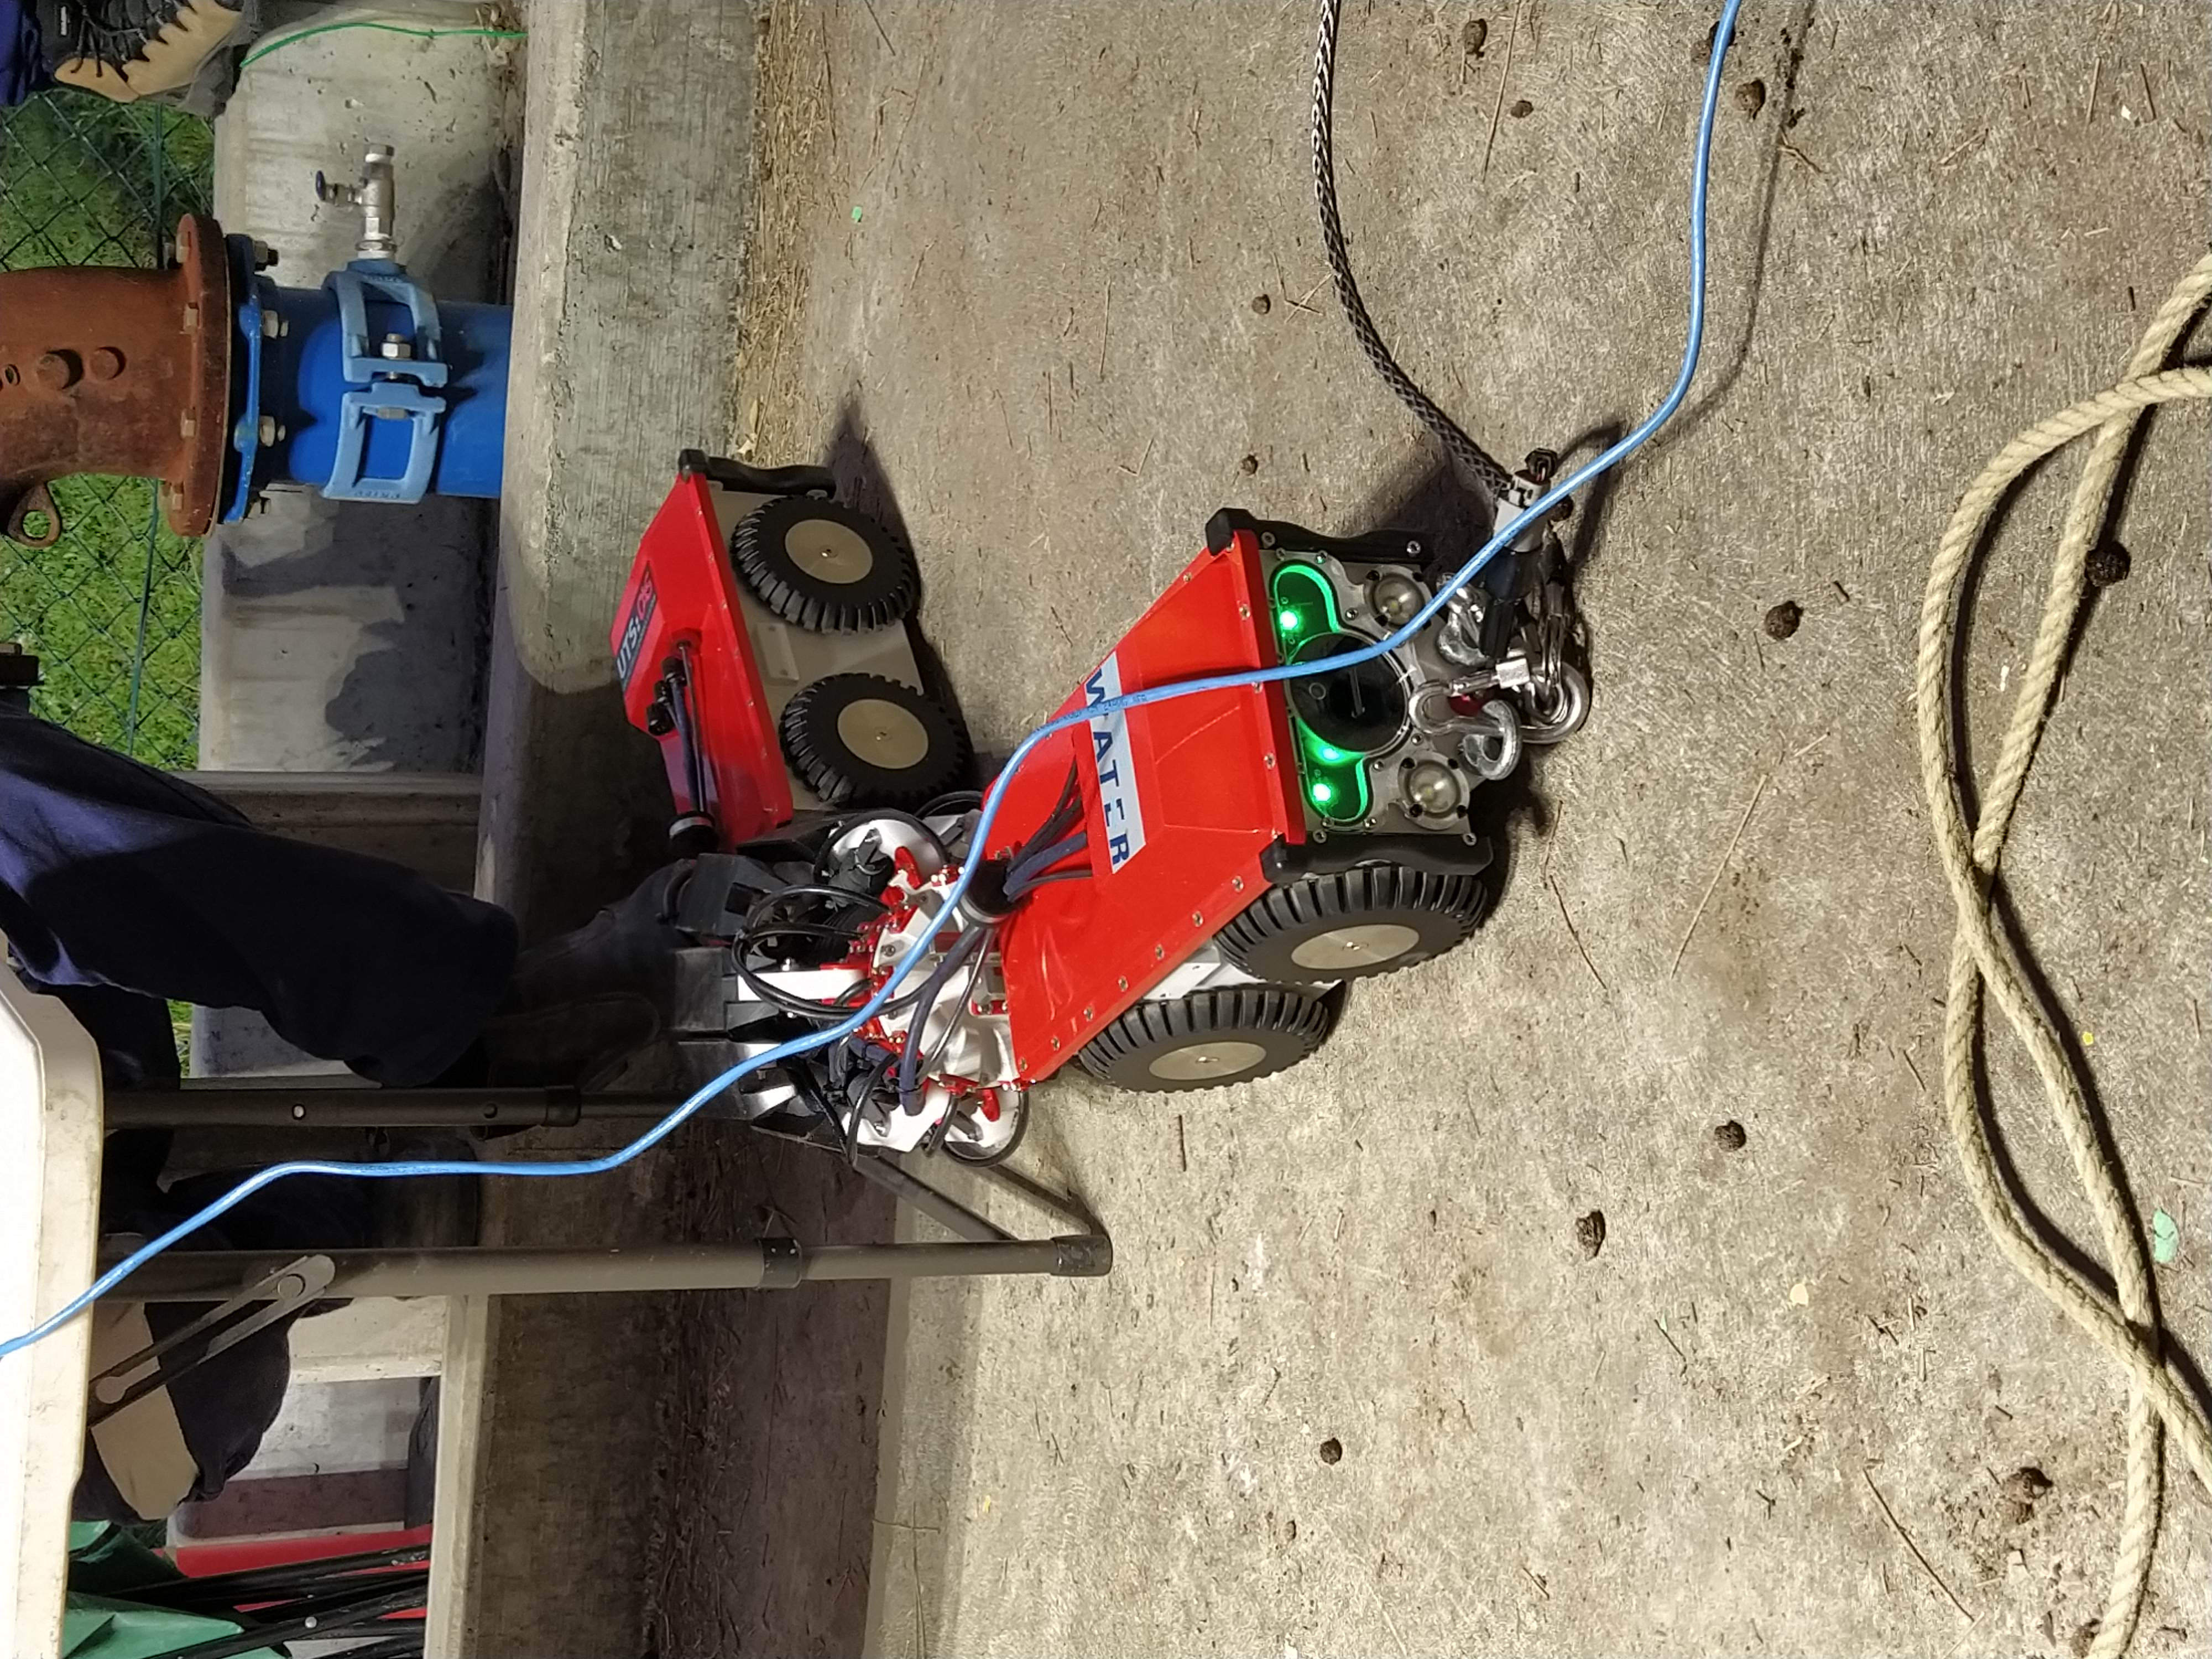
\includegraphics[angle=90, width=\textwidth]{images/rima2/RIMA2_Physical.png}
        \caption{RIMA2}
        \label{fig:rima2}
    \end{minipage}
\end{figure*}

% Tether Protetiion Section
\newpage
\subsection{Mechanical Work}

\textbf{Utilities for RIMA1 and RIMA2 Field Trials:} I designed a number of utilities to assist with field trial deployments to prevent damage to equipment and site. Using solidworks I designed
tether protection for flangless and flanged pipes [~\ref{fig:tethproc}] which were later manufactured to be used in deployments. The tether protection units are designed with the following intent:

\begin{itemize}
    \item Ease of use for Sydney Water personnel
    \item Prevent damage to the tether and pipe wall at entrance where edge is sharp
    \item Adjustability for different pipe diameters (250mm to 750mm)
    \item Stainless steel for Chemical and Weather resitance and durability
    \item Simple lock-pin mechanism to ensure ease of use when wearing gloves
    \item Teflon block with internal radius matched to the bend radius of tether cable connected from base station to the robot
    \item Simple, low cost design
\end{itemize}

\imgpairin{utility/flangless_tether_protection.JPG}{Flangless Tether Protection}{utility/tether_protection_flanged.JPG}{Flanged tether protection}{Tether Protection}{tethproc}{90}{270}

% Deployment Cradle Section
\newpage

The next utility I designed was a debloyment cradle for RIMA2 [~\ref{fig:jdm}]. Often, due to safety constraints only one person is allowed into the sewer pit. This does not favour the handling of RIMA2 which is a 3-body 
system best carried and inserted into pipes safely by two people. After an incident in a previous deployment before I started where RIMA2 was dropped, I was assigned with designing a cradle. The advantage 
of the cradle to safely lower and deploy RIMA2. The final deisgn has the following features:

\begin{itemize}
    \item Can be lowered using block-and-chain or cranes (varies with resource availability on site)
    \item Lightweight to ensure weight requirements are met as per agreement with Sydney Water
    \item Simple, intuitive locking mechanisms to ensure ease of use for Sydney Water personnel
    \item Custom flange design to adapt to various flanged pipe diameters (250mm to 450mm) if additional support is required
\end{itemize}

\imgpairin{utility/jdm.jpg}{RIMA2 Cradle in lab}{utility/jdm_in_use.jpg}{Cradle in use on field trial}{RIMA2 Cradle}{jdm}{0}{270}

% Rollover-Assist RIMA1
\newpage
\textbf{RIMA1 Rollover Assist:} I designed a set of rollover assist devices for RIMA1 after an incident in one of the first trial runs with Sydney Water having full control in our robot when unfortuntaely
a software bug caused the robot to drive autonomously up the pipe wall causing in to invert. The aim of the rollover assist is to assist in manually having to pull the robot out the pipe when it inverts, as 
using mchinery to dig up the robot can be costly, time-consuming and potentially impossible depending on location.The inital inspiration [~\ref{fig:rp}] actually came from when I pulled apart my skateboard and attached it to RIMA1.
The final design [~\ref{fig:fdra}] after a few iterations is quite different from this and is simply a modification of the Sensor Pad on the sensor head with a custom bracket that could be fitted to RIMA1 with a simple modification to the handles.  

\imginin{rima1/rollover_prototype.jpg}{Rollover Prototype}{rp}{0.29}
\imgpairin{rima1/rollover_rear.jpg}{Rollover Assist Rear View}{rima1/rollover_side.jpg}{Rollover Side View}{Final Design Rollover Assist}{fdra}{270}{0}

\subsection{Electrical Work}

% RIMA1 System Board Instalation
\textbf{RIMA1 System Board Installation:}

% RIMA2 New PEC Board Test Rig
\newpage
\textbf{RIMA2 New PEC Board Test Rig:}

% RIMA2 New PEC Board Installation
\newpage
\textbf{RIMA2 New PEC Board Installation:}


% RIMA2 Debugging
\newpage
\textbf{RIMA2 Electrical Debugging:}
\newpage
\subsection{Software Work}

% Give a brief software overview
\textbf{Software Brief: }
RIMA1 and RIMA2 ran off the ROS1 Melodic framework. They utilised custom messages and customised ROS packages to function. All code for the robot was written in C++ and analysis scripts used for PEC are written
in Python. Unfortunately the codebases for these robots cannot be shared as it is property of UTS and Sydney Water. The robots processes and GUI's are all run/launched ushing shell scripts in the linux CL.

% New RIMA1 system board software update
\vspace{\baselineskip}
\textbf{RIMA1 System Board Software Update: }
The new system board required some minor software updates. This primarily consisted of changes to message data types and names. This change also required small modification to RIMA1's core.cpp file which was resposible 
for ROS handling (i.e. setting up subscribers, publishers, etc.). 

% RIMA1 GUI Update
\vspace{\baselineskip}
\textbf{RIMA1 GUI Update: }
The old GUI of RIMA was outdated and not greatly designed and doing something simple such as turning required going into settings and modifying rotation setpoints which is clearly not ideal or user friendly. I updated
the GUI [~\ref{fig:r1gui}] to have more intuitive control, I also installed rear cameras at the time for rear view and visual view of the sensor to have a better cue of full expansion rather than basing it off the current reading. Basic 
IMU visualisation was also added to the GUI to allow for better understanding of the robot's orientation in the pipe. The GUI was written in C++ using Qt Designer.

\begin{figure*}[htbp]
    \centering
    \subfloat[Old RIMA1 interface]{
        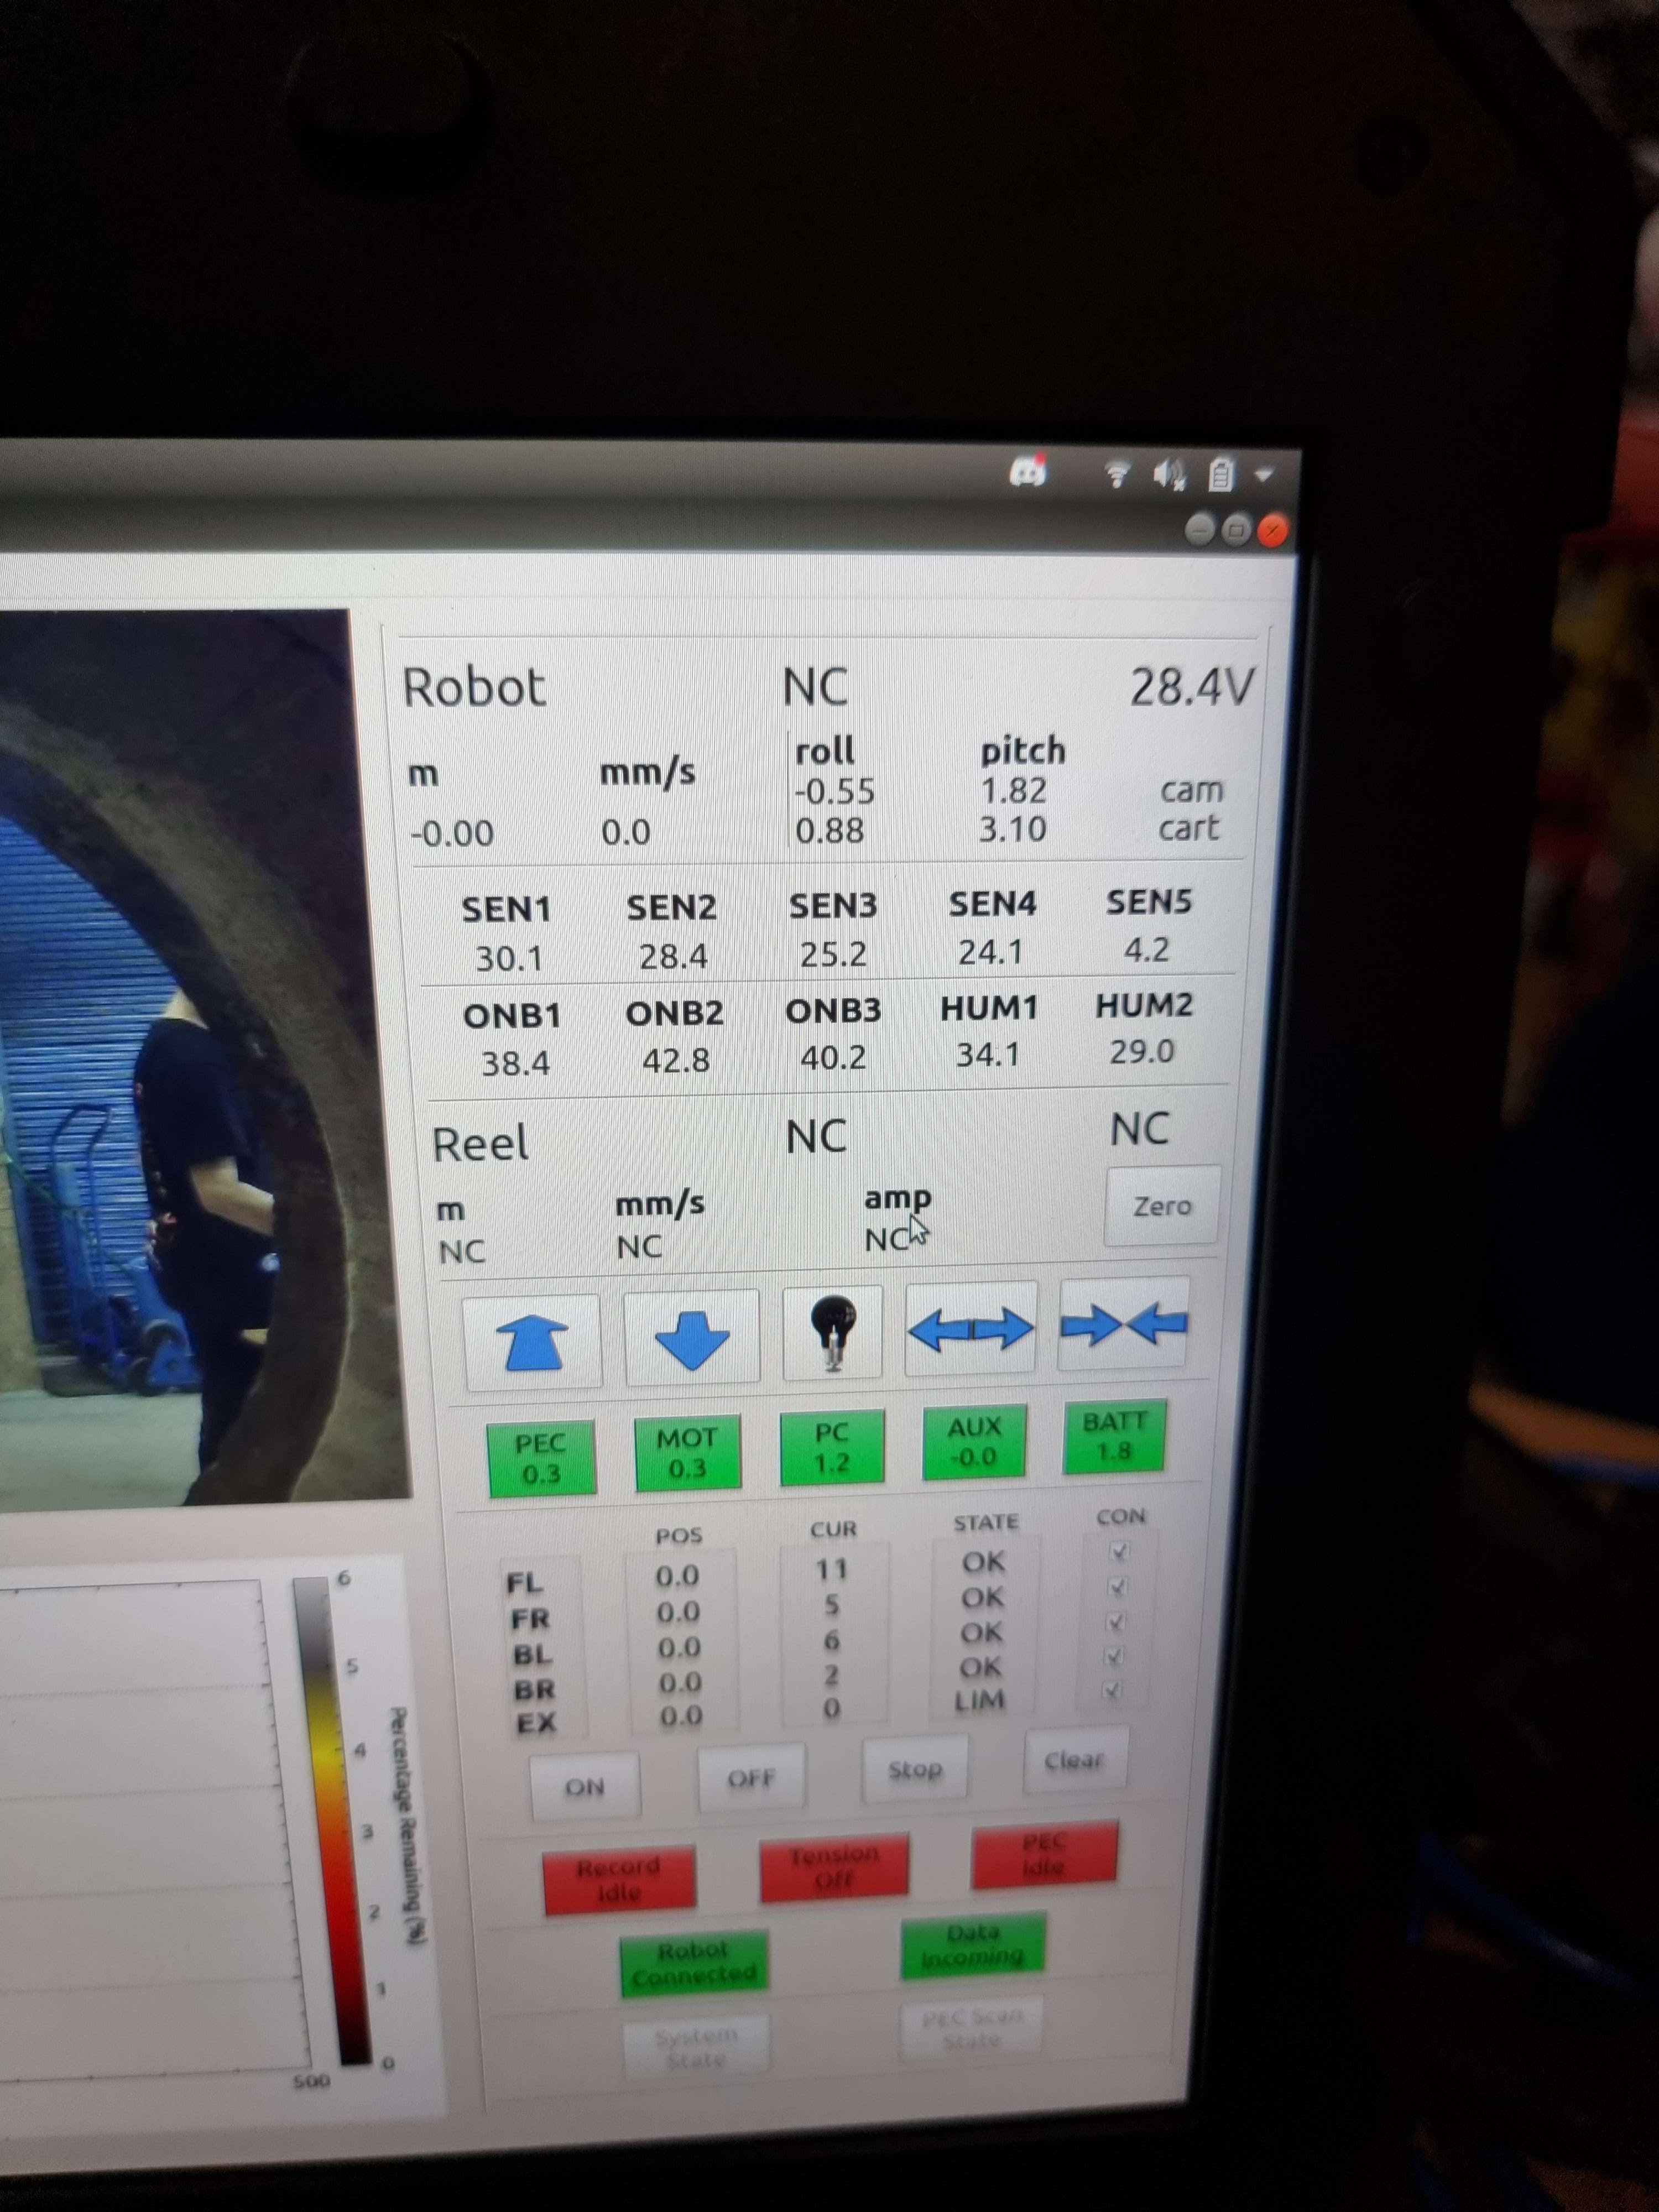
\includegraphics[width=0.30\textwidth, valign=c]{images/rima1/rima1_old_gui.jpg}
    }
    \hspace{0.5cm}
    \subfloat[New RIMA1 interface]{
        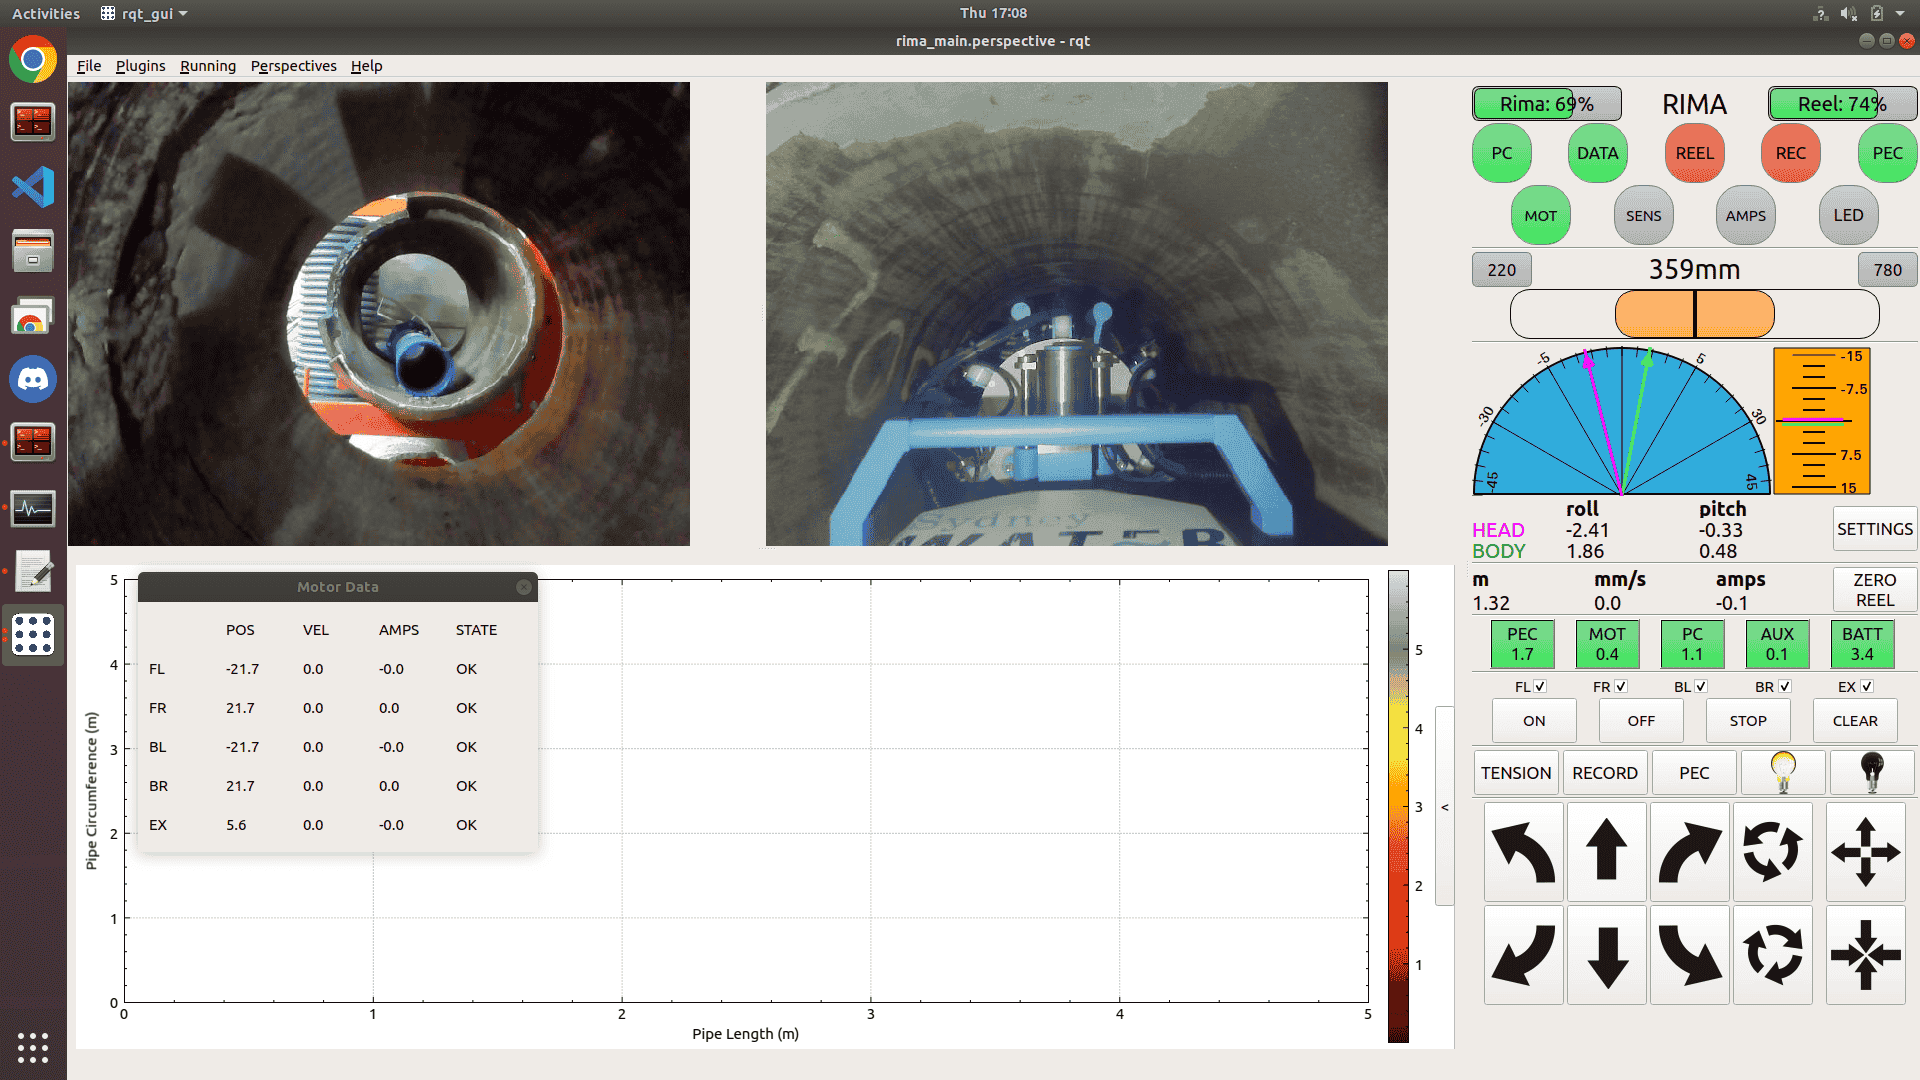
\includegraphics[width=0.60\textwidth, valign=c]{images/rima1/rima_gui_new.png}
    }
    \caption{Comparison of RIMA1 GUI's}
    \label{fig:r1gui}
\end{figure*}
\newpage
\imginin{rima1/rear_cam_rear.jpg}{RIMA1 Rear Camera rear View}{rcam}{0.8}

% Embedded software debugging for RIMA2 PEC

% PEC Calibration

% Simplified shell script for data tranfer
   
\newpage
\section{S100: Demonstartion robot for the UTS Robotics Institute} 
\label{sec:s100}
The S100 demonstration robot [~\ref{fig:s100}] is an incomplete project before my departure from the UTS Robotics Institute. It was a robotic platform smaller than RIMA2 intented to do similar tasks to the RIMABOT Project. The robot
was desiged with the following featrures:

\begin{itemize}
    \item Single Teensy MCU for control
    \item Communicated with base station using an MQTT broker over ethernet to replicate similar communcation functionality to RIMA1 and RIMA2
    \item GUI with intuitive controls and a 3D real-time imu visualisation devolped using ReactJS [~\ref{fig:s100gui}]
    \item The ability to be used without ROS to make it more user friendly for non-technical users
    \item The GUI was also linux compatible and a ROS bridge could be used to also control the Robot in ROS amongst other things, making the robot versatile for both general and research use. The React application
itself would generate all ROS topics using standard ROS packages if the ROS bridge was used.
\end{itemize}

\textbf{Codebase: } The repository for the S100 project can be found \href{https://github.com/jackfruittt/S100_Interface}{here}

\newpage
\imginin{s100/s100_robot.png}{S100 Robot}{s100}{0.4}
\imginin{s100/webui.png}{S100 GUI}{s100gui}{0.8}
\newpage
\section{Course Work}
\label{sec:course_work}

\textbf{Brief: } This section will go over the course work I have done throughout my degree throughout various subjects that I'm quite proud of and believe are industry relevant. The projects will go in chronological
order of when I completed them.

\subsection{Mechanical/Mechatronic Work}

\subsubsection{MDFS Robot for Warman Challenge:}

\textbf{Subject: } Mechhanical Design Fundamentals Studie 1 (Spring 2023) \newline
\textbf{Grade Achieved: } Distinction \newline
\textbf{Project Overview: }
The goal of the assignment was to design an autonomous robot [~\ref{fig:beepboop}] that could traverse a track to collect tennis balls and deposit them into a Silo [~\ref{fig:render}]. The final robot my team produced was successful in making the leaderboard.
Below are my contributions to the final design of the project:

\begin{itemize} 
    \item Full electrical design [~\ref{fig:sheet1}] [~\ref{fig:sheet2}] with safety features fuses and properly rated components
    \item Custom designed 3D printed TPU Wheels [~\ref{fig:wheel}]
    \item Chassis design and calculations
    \item Parrallel Manipulator design 
    \item Software design and implementation
    \item Construction of the robot
\end{itemize}

Whilst this looks like I did everything, it's important to clarify that my group did contribute to different designs for various sub-systems however, the sub-systems didn't integrate together well and we had two members 
(it was a five person group including myself) not contribute for the semester. Because a last minute redesign
was needed we agreed as a team that I would take over the entire design of the robot given my experience and they would focus on the group documentation and the presentation which was a large component along with the robot. Without their efforts in this, I would
not have achieved the grade I did.

\imgpairin{mdfs/wheel_side_view.png}{CAD model of wheel}{mdfs/wheel_printed}{Wheel being printed with TPU}{Wheel Design}{wheel}{0}{0}
\imginin{mdfs/Sheet_1.png}{Power distribution Circuit}{sheet1}{0.8}
\imginin{mdfs/Sheet_2.png}{MCU circuit}{sheet2}{0.8}
\imginin{mdfs/robot_render_on_track.png}{Robot Render}{render}{0.8}
\imginrot{mdfs/final_robot.JPG}{Final Robot}{beepboop}{0.5}{270}
\newpage
\subsection{Electrical Work}

\subsubsection{Low Level Circuit Design using Keysight ADS:}
\textbf{Subject: } Microelectronics (Autumn 2025) \newline
\textbf{Grade Achieved: } High Distinction (88) \newline
\textbf{Project Overview: }
Over the semester, I designed three low level circuits that had to meet certain specifications. I designed a Low Pass Filter (LPF), a Balun Circuit and a Low Noise Amplifier (LNA).
This type of circuit design differs from standard circuit design as it uses unideal components where noise and resonance effects are taken into account. All components are tuned at
a low level. For example, an inductor is not simply assigned an inductance value, instead its parameters such as coil length, spacing, number of turns, etc. are set instead. This is necessary 
for high speed circuit design where the slightest change in just one of these parameters can effect the entire circuit. 

% LPF
\subsubsection{LPF:}

\textbf{Benchmark Specifications: }

\begin{table}[htbp]
\centering
\begin{tabularx}{\textwidth}{@{} l l X @{}}
\toprule
\textbf{Parameter} & \textbf{Symbol} & \textbf{Value} \\
\midrule
Centre frequency & $f_0$ & 2.5 GHz \\
Insertion loss & IL & < 2 dB \\
Return loss (both ports) & RL & > 10 dB \\
Bandwidth & FBW & 30–50\% \\
Out-of-band rejection & OoB & > 30 dB at $2f_0$ \\
\bottomrule
\end{tabularx}
\caption{Filter Design Specification}
\end{table}

\newpage
\textbf{Result Delivered: }

\begin{table}[htbp]
\centering
\begin{tabular}{l l c}
\toprule
\textbf{Specification parameter} & \textbf{Result delivered} & \textbf{Spec met?} \\
\midrule
Centre Frequency (2.5 GHz) & 2.75 GHz & \cmark \\
Insertion Loss & < 2 GHz & \cmark \\
Return Loss (Both Ports) & > 10 dB & \cmark \\
Fractional Bandwidth & 61\% & \xmark \\
Out-of-band rejection & 15/18 dB (assignment/actual $f_c$) & \xmark \\
\bottomrule
\end{tabular}
\caption{Benchmark Results}
\end{table}

\newpage
\textbf{Circuit Design:}
\imginin{micro/lpf_circuit.png}{Low Pass Filter Circuit Design}{lpf}{0.8} \newline
\textbf{Simulation Results: }
\imginin{micro/lpf_sim.png}{Low Pass Filter Simulation}{lpfsim}{0.6}

% Balun
\newpage
\subsubsection{Balun:}

\textbf{Benchmark Specifications: }

\begin{table}[htbp]
\centering
\begin{tabularx}{\textwidth}{@{} l l X @{}}
\toprule
\textbf{Parameter} & \textbf{Symbol} & \textbf{Value} \\
\midrule
Centre frequency & $f_0$ & 15 GHz (±10\%) \\
Balanced output load impedances & $Z_L$ & 30 Ohms \\
Unbalanced source impedance & $Z_s$ & 50 $\Omega$ \\
Amplitude balance over FBW & AB & ± 0.5 dB \\
Phase balance over FBW & PB & ± 3\textdegree \\
Insertion loss (for both outputs) & IL & 3 - 4 dB \\
Return loss (for input port) & RL & > 10 dB \\
Bandwidth & FBW & > 15\% \\
\bottomrule
\end{tabularx}
\caption{Design specifications for Balun}
\end{table}


\textbf{Result Delivered: }

\begin{table}[htbp]
\centering
\begin{tabular}{l l c}
\toprule
\textbf{Specification parameter} & \textbf{Result delivered} & \textbf{Spec met?} \\
\midrule
Cf & 54.25 GHz (target 55 GHz) & \cmark \\
AB & -0.495 – -0.221 & \cmark \\
PB & -7.453, -9.180 & \xmark \\
IL & -3.743, -3.998 & \cmark \\
RL & -19.841 dB & \cmark \\
FBW & (66.25 – 39.75)/55 * 100 = 48.18\% & \cmark \\
\bottomrule
\end{tabular}
\caption{Benchmark Results}
\end{table}

\newpage
\textbf{Circuit Design:}
\imginin{micro/balun_circuit.png}{Balun Circuit Design}{balun}{0.8}
\newpage
\textbf{Simulation Results: }
\imginin{micro/balun_sim.png}{Balun Circuit Simulation}{balunsim}{0.7}

% LNA
\newpage
\subsubsection{LNA:}

\textbf{Benchmark Specifications: }

\begin{table}[htbp]
\centering
\begin{tabularx}{\textwidth}{@{} l l X @{}}
\toprule
\textbf{Parameter} & \textbf{Symbol} & \textbf{Value} \\
\midrule
Centre frequency & $f_0$ & 15GHz \\
Noise Figure & $nf$ & < 1.2 dB \\
Transducer Power Gain & $TPG$ & > 10 dB \\
Return Loss (Input and Output) & RL & > 10 dB \\
Quiescent DC Power Consumption & QDP & < 0.2W \\
\bottomrule
\end{tabularx}
\caption{Design specifications for LNA}
\end{table}


\textbf{Result Delivered: }

\begin{table}[htbp]
\centering
\begin{tabular}{l l c}
\toprule
\textbf{Specification parameter} & \textbf{Result delivered} & \textbf{Spec met?} \\
\midrule
Cf & 15 GHz & \cmark \\
Nf & 0.890 dB & \cmark \\
TPG & 11.557 dB & \cmark \\
RL & 11.336 dB, 11.693dB & \cmark \\
QDP & 0.14385 W & \cmark \\
\bottomrule
\end{tabular}
\caption{Benchmark Results}
\end{table}

\newpage
\textbf{Circuit Design:}
\imginin{micro/lna_circuit.png}{LNA Circuit Design}{lna}{0.8} \newline
\textbf{Simulation Results: }
\imginin{micro/lna_sim.png}{LNA Circuit Simulation}{lnasim}{0.8}

\newpage
\subsection{Software Work}

% Wii Wii and Mii
\subsubsection{Wii Wii and Mii: Cooking Cobots}
\textbf{Subject: } Industrial Robotics (Spring 2024) \newline
\textbf{Grade Achieved: } Distinction \newline
\textbf{Project Overview: }
The aim of this project was to work in pairs and have two robot manipulators of our choice working in any environment of our choosing, and simulate the task in MATLAB or Python. My team chose the PR2 (Wii Wii) and TM5700 (Mii) [~\ref{fig:cobot}].
For this assignment we wanted have a cooking cobot pair. I developed all logic for the PR2 and some of the TM5, whilst my partner handled majority of the TM5 code. I managed the codebase for this project to ensure code structure was the same to 
make merge requests in GitHub and testing easier. The simulation is programmed in matlab and 
contains the following features:

\begin{itemize}
    \item PR2 utilising a total of 15 DOF
    \item TM5700 using 6 DOF
    \item Cubic spline trajectory
    \item Trajectory generation using waypoints
    \item Functional 2D LiDAR simulation for the PR2 to detect objects
    \item GUI for the PR2 for manual control using sliders
    \item Collision detection (in GUI only)
    \item Custom controller for the TM5 to control it manually
    \item Usage of both forwards and inverse kinematics 
    \item Usage of the pseudo-inverse jacobian for the PR2
    \item Hybrid control system for the PR2 (using Cartesian Trajectory and IK)
    \item Hybrid control system for the TM5 (using RMRC and IK)
    \item PR2 and TM5 working together to prepare food
\end{itemize}

\textbf{Codebase: } \href{https://github.com/jackfruittt/Industrial_Robotics_A2}{Code here} \newline
\textbf{Video Demonstration: } \href{https://www.youtube.com/watch?v=JsQmZcRGo9Y}{Project Trailer} and \href{https://youtu.be/irytygtPb94}{project demonstration} \newline

Another component of this project was to control an actual robot using Python or MATLAB. We chose to control the TM5 using Python via ROS Noetic which I wrote the code for. 
Code can be found \href{https://github.com/jackfruittt/tm5_ros_python}{here}.

\imginin{ir/wiiwiimii.png}{Wii Wii and Mii}{cobot}{0.5}



% PFMS
\newpage
\subsubsection{Autonomous Terrain Surveying Drone}
\textbf{Subject: } Programming for Mechatronic Systems (Autumn 2025) \newline
\textbf{Grade Achieved: } Distinction (82) \newline
\textbf{Project Overview: }
The aim of this projectg was to develop an autonomous drone [~\ref{fig:drone}] that could survey terrain using the ROS2 Humble framework and only standard ROS Packages. This was fully written is C++
using proper OOP principles. The project also has supporting documentation using Doxygen. The key features of this project are:

\begin{itemize}
    \item Sonar sensor for terrain mapping and alitude control
    \item 2D LiDar for obstacle detection
    \item Asymmetric PI controller for altitude controller (always 2m above relative terrain)
    \item Gradient map produced using finite difference method
    \item 1D Kalman filter for gradient map smoothing if revisiting visited cells
    \item Live gridmap area updates based on flight path for optimisation
    \item Shell scripts to automate process of recording rosbags
    \item Unit tests using Google Test Framework which utilise rosbag data
    \item Threading for multiple drone operation
    \item Waypoint visualisation
\end{itemize}

\textbf{Codebase: } \href{https://github.com/jackfruittt/Terrain-Surveying-Drone}{Code here} \newline

\imginin{pfms/drone.png}{Terrain Surveying Drone}{drone}{0.5}

More information about how the project works and runs can be found in the doxgen documetation. The doxygen components are pre-built and the repo goes over how to launch the index.html file.
Note: There are more projects for this subject however, they're simply projects to help build to this assigment and my code is wirtten the same throughout so i've decided not to include them.


\end{document}